
\thispagestyle{empty}

\begin{center}
\Large
%Introduction
Préambule
\normalsize
\end{center}
\vspace{3cm}

Ce document est une compilation d'articles provenant de deux
ouvrages : {\it La pratique de la philosophie} destiné aux
lycéens, une encyclopédie de la philosophie destinée aux néophytes.

(Complété par un dictionnaire encyclopédique de poche et un
dictionnaire étymologique pour l'article {\it vérité.})

Il souhaite donner un aperçu élémentaire et succinct de la
philosophie à propos de la croyance et de la vérité.

%\vspace{1.3cm}
\vfill

\begin{center}
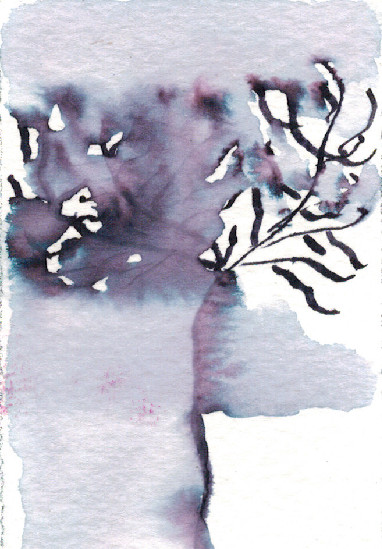
\includegraphics[scale=0.5]{./presentation/gauche2}
\hspace{1cm}
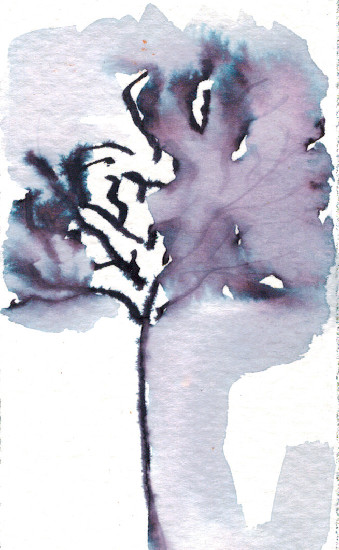
\includegraphics[scale=0.5]{./presentation/droite2}
\end{center}

%« Chaque fois que les gens s’interrogent "Mais qu’est-ce donc que la vérité ?" – en général, c’est parce que la vérité est juste sous leur nez, mais il serait fort incommode d’en convenir. Et aussi, à l’encontre de sa conviction intime, Pilate cède à la volonté de la foule et lui abandonne Jésus pour qu’il le crucifie. Le problème pour Pilate n’était pas déterminer si Jésus était innocent. Cette question-là était facile à trancher. Non, le vrai problème est que, en fin de compte – comme nous tous, la plupart du temps –, la vérité était devant lui, mais il a préféré s’en laver les mains. »

%Simon Leys, Le bonheur des petits poissons. Lettres des Antipodes, éd. JC. Lattès, 2008
%\vspace{2.3cm}
\vfill

\hfill Numérisation : Stephan Runigo

\hfill Illustrations : Krikri

%%%%%%%%%%%%%%%%%%%%%%%%%%%%%%%%%%%%%%%%%%%%%%%%
